\subsection{Боксплот Тьюки}
\label{subsec:result_boxplot}
\begin{itemize}
	\item{Нормальное распределение}
	\begin{figure}[H]
		\begin{center}
			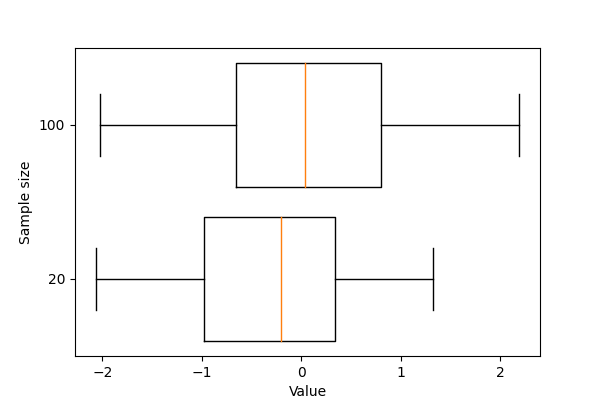
\includegraphics[scale=0.75]{part_boxplot/figures/normal}
			\caption{Боксплот Тьюки Нормальное распределение}
			\label{fig:boxplot_normal}
		\end{center}
	\end{figure}
	
	\item{Распределение Коши}
	\begin{figure}[H]
		\begin{center}
			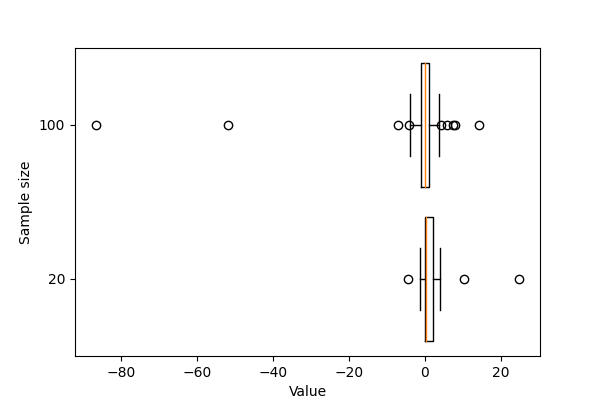
\includegraphics[scale=0.75]{part_boxplot/figures/cauchy}
			\caption{Боксплот Тьюки Распределение Коши}
			\label{fig:boxplot_cauchy}
		\end{center}
	\end{figure}
	
	\item{Распределение Лапласа}
	\begin{figure}[H]
		\begin{center}
			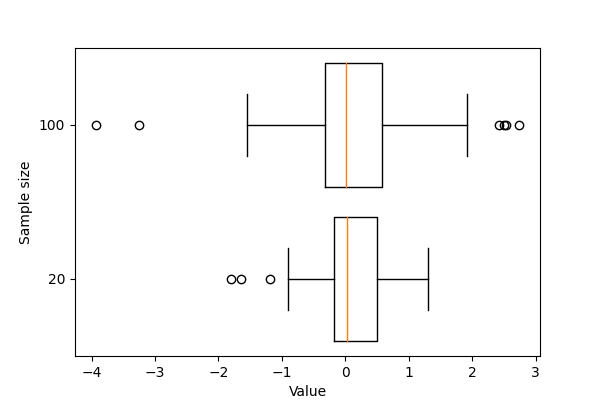
\includegraphics[scale=0.75]{part_boxplot/figures/laplace}
			\caption{Боксплот Тьюки Распределение Лапласа}
			\label{fig:boxplot_laplace}
		\end{center}
	\end{figure}
		
	\item{Распределение Пуассона}
	\begin{figure}[H]
		\begin{center}
			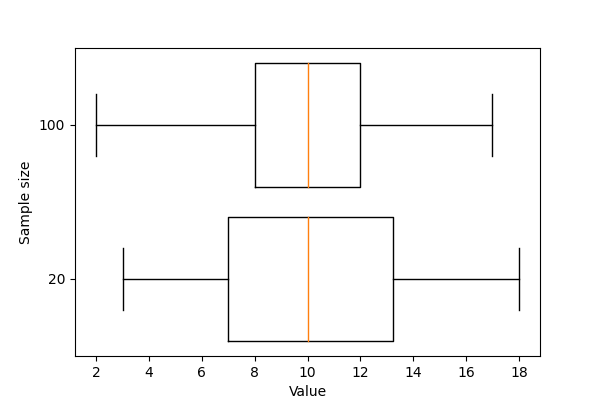
\includegraphics[scale=0.75]{part_boxplot/figures/poisson}
			\caption{Боксплот Тьюки Распределение Пуассона}
			\label{fig:boxplot_poisson}
		\end{center}
	\end{figure}
	
	\item{Равномерное распределение}
	\begin{figure}[H]
		\begin{center}
			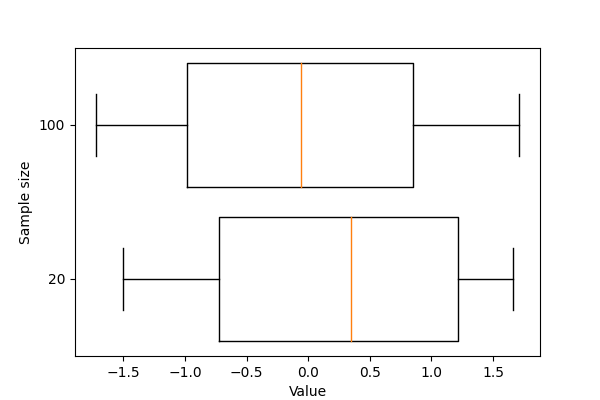
\includegraphics[scale=0.75]{part_boxplot/figures/uniform}
			\caption{Боксплот Тьюки Равномерное распределение}
			\label{fig:boxplot_uniform}
		\end{center}
	\end{figure}

\end{itemize}

\subsection{Доля выбросов}
\label{subsec:result_outliers_fraction}
Выборка случайна, поэтому в качестве оценки рассеяния можно взять дисперсию пуассоновского потока: $D_n \approx \sqrt{n}$ \newline
Доля $p_n = D_n / n = 1 / \sqrt{n}$ \newline
Доля $n = 20$: $p_n = 1 / \sqrt{20}$ - примерно 0.2 или 20\% \newline
Доля $n = 100$: $p_n = 1 / 10$ - 0.1 или 10\% \newline
Из этого можно решить, сколько знаков оставлять в доле выбросов. \newline

\begin{table}[H]
	\centering
		\begin{tabular}[t]{|l|r|}
			\hline
			Выборка & Доля выбросов\\
			\hline
			Normal n = 20   &  0.02\\
			\hline
			Normal n = 100   &  0.01\\
			\hline
			Cauchy n = 20   &  0.15\\
			\hline
			Cauchy n = 100   &  0.15\\
			\hline
			Laplace n = 20   &  0.08 \\
			\hline
			Laplace n = 100   &  0.07 \\
			\hline
			Poisson n = 20   &  0.02 \\
			\hline
			Poisson n = 100   &  0.01 \\
			\hline
			Uniform n = 20   &  0\\
			\hline
			Uniform n = 100   &  0\\
			\hline
		\end{tabular}
		\caption{Доля выбросов}
		\label{tab:experimental_fraction_of_outliers}
	\end{table}
	
\subsection{Теоретическая вероятность выбросов}
\label{subsec:result_outliers_probability}
    \begin{table}[H]
	    \centering
		\begin{tabular}[t]{|l|r|r|r|r|r|}
			\hline
			Распределение   &      $Q_1^T$	& $Q_3^T$ & $X_1^T$ & $X_2^T$ & $P_B^T$	\\
			\hline
			Нормальное распределение 	& -0.674& 0.674 & -2.698 	&  2.698 	& 0.007 \\
			\hline
			Распределение Коши 			& -1	& 1		&  -4		& 4			& 0.156 \\
			\hline
			Распределение Лапласа 		& -0.490& 0.490	& -1.961	& 1.961		& 0.063 \\
			\hline
			Распределение Пуассона 		& 8		& 12	& 2			& 18		& 0.008 \\
			\hline
			Равномерное распределение 	&-0.866 & 0.866	& -3.464 	& 3.464 	& 0	\\
			\hline
		\end{tabular}
		\caption{Теоретическая вероятность выбросов}
		\label{tab:theoretical_probability_of_outliers}
\end{table}